



\chapter{UX Design}
\begin{flushleft}
	\textit{Quali processi e metodi utilizzare per portare avanti il progetto di un
		prodotto software?}
\end{flushleft}

In questo capitolo si analizzeranno diversi processi.
Essi non vanno identificati come fasi ben definite e statiche, da seguirsi una dietro l'altra, bensì come \textbf{fasi} \textbf{dinamiche} e \textbf{alternabili}.

\section{Personas}
Identificato correttamente il problema mediante la \textbf{Task Analysis}, come si  possono creare elementi individuali? Come si identificano le così dette le \textbf{Personas}?

\begin{figure}[!h]
	\centering
	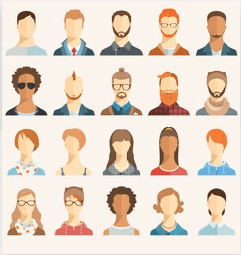
\includegraphics[scale=0.55]{immagini/Personas.png}
\end{figure}

Il primo passo da fare dopo la Task Analysys è \textbf{identificare le personas}.
Una \textbf{personas} è l'\textbf{archetipo di uno dei possibili utenti}. Scrivere e
identificare le personas aiuta a colmare la distanza tra il cliente e l'azienda, in modo da capire cosa vuole e cosa si aspetta l'utente dal prodotto, ma anche cosa gli crea frustrazione nell'usarlo. Esistono molte \textbf{tecniche} atte a fare fare un'analisi degli utenti e che aiutano i progettisti a identificare e a scrivere le personas:

\begin{itemize}
	\item \textbf{Task Analysis}.
	\item \textbf{Feedback} tra i quali: analisi delle attività, interviste e focus groups.
	\item \textbf{Prototipazione}.
\end{itemize}

Sorge spontanea la domanda seguente: \textit{ma quante personas è bene definire}?
Per rispondere a questa domanda ci si basa sul \textbf{Principio di Pareto}: \begin{center}
	\textit{Concentrarsi sul 20\% degli utenti che utilizzerà il prodotto per l'80\% dell'uso complessivo.}
\end{center}

\pagebreak

\section{Requirements}

Un \textbf{requirement} è un servizio o una caratteristica che soddisfa un bisogno di un utente.
I requirements possono essere funzioni, vincoli, regole aziendali o altri tipi di elementi di cui il prodotto deve essere dotato per soddisfare le esigenze degli utenti. È quasi ovvio che trovare i \textbf{requirements corretti} risulta molto più \textbf{semplice} se in precedenza sono state \textbf{individuate} e \textbf{descritte} le \textbf{personas}.

Infatti è controproducente scrivere anticipatamente i requirements,
è complesso se non impossibile descriverli tutti all'inizio di una fase di progettazione. Risulta più facile descrivere i requirements con l'avanzamento del progetto, in modo da poter capire come modificare, eliminare o aggiungere i requirements giusti, tenendo in considerazione anche le personas a cui è destinato il prodotto finale.

Il \textbf{requirements driven development} è un approccio complesso e oneroso e va in \textbf{contrasto} con il metodo \textbf{Agile} che richiede si sia sempre pronti al cambiamento. Questo approccio così poco flessibile sta andando sempre meno di moda tuttavia è bene seguirlo una volta definiti i requirements per quel 20\% di software che utilizzerà l'80\% delle personas.

Esistono \textbf{due tipi di requirements} per il mondo della UI:

\begin{itemize}
	\item \textbf{Funzionali}:
	      descrivono quali funzionalità deve avere il software. Rispondono alla domanda:
	      \textit{Cosa fa?}
	\item \textbf{Non funzionali}: specificano i tratti qualitativi del prodotto. Rispondono alla domanda: \textit{Come lo fa?} e descrivono inoltre
	      attributi come sicurezza affidabilità e manutenibilità.
\end{itemize}

\section{User Stories}
Dopo aver definito \textbf{personas} e \textbf{requirements}, il prossimo passo è la scrittura delle \textbf{User Stories}.

Una \textbf{user story} è una breve descrizione che identifica l'utente insieme al suo
obiettivo e alle sue necessità, determina \textbf{chi è}, \textbf{di cosa ha bisogno e perché ne ha bisogno}. Tipicamente ci sono una o più user stories per ogni personas, ma \textbf{non il contrario}: avere più personas per una user story significa aver descritto la medesima persona con termini differenti e quindi averne introdotta una ridondante.
Se una user story non copre tutte le sfaccettature della singola persona che dovrebbe descrivere è indizio del fatto che tale persona potrebbe essere troppo \textbf{ampia}, ed è bene che venga suddivisa in più personas.

Una user story è un \textbf{requirement} espresso \textbf{dalla prospettiva del cliente}.

Con le user stories si ottengono due importanti risultati: si \textbf{migliorano le descrizioni delle personas}, migliorandone il dettaglio e arricchendole con una narrativa, e si ha un elemento tangibile per valutare lo sviluppo del prodotto e fare il punto della situazione.
Esiste uno schema ben preciso per scrivere una user story:

\begin{center}
	\textbf{\large As a [role], I want [feature] because [reason]}
\end{center}

\begin{flushleft}
	\textit{Chi scrive le user stories?}
\end{flushleft}

\textbf{Tutti}! È responsabilità del proprietario del prodotto assicurarsi che vengano scritte delle stories giuste e corrette, ma non significa che le debba
scrivere lui stesso. Nel corso di un buon progetto Agile ci si aspetta che ogni membro del team partecipi alla scrittura delle user stories secondo un \textbf{metodo collaborativo}.

\pagebreak

\begin{flushleft}
	\textit{A che livello è bene scriverle?}
\end{flushleft}

Uno dei grandi benefici delle user stories è che possono essere
scritte a \textbf{vari livelli di dettaglio}.

Possiamo avere user story di livello \textbf{epic}, ovvero in grado di
coprire un grande quantità di funzionalità, tipicamente sono disutili ma possono diventare interessanti se spacchettate in user stories più piccole e, di conseguenza, più dettagliate. Una \textbf{user story epic} può essere \textbf{divisa} in decine o centinaia di user stories più piccole.

I dettagli possono essere aggiunti sostanzialmente in due modi:
\begin{enumerate}
	\item Suddividendo una user story in user stories più piccole e quindi più dettagliate.
	\item Aggiungendo \textbf{condizioni di soddisfacimento dell'utente}, ovvero  dettagli che contribuiscono al grado di soddisfacimento dell'utilizzatore del prodotto, suddividendole per ogni eventuale membro di soddisfacimento. Quest'ultima è una tecnica molto difficile da utilizzare nel mondo della progettazione software.
\end{enumerate}

\section{Scenarios}

Gli \textbf{scenarios} sono l'\textbf{evoluzione delle user stories}. Una user story sintetizza in brevi frasi cosa fa l'utente con il software e quale bisogno deve soddisfare.

Lo \textbf{scenario estende la user story} andando a descrivere anche quali motivazioni hanno portato l'utente ad usare il software e come egli si comporterà nel suo utilizzo. Inoltre gli scopi o \textbf{goals} delle personas vengono \textbf{estesi} e descritti in maniera più ampia.

\begin{flushleft}
	\textit{Ma a cosa serve uno scenario?}
\end{flushleft}

Le \textbf{user stories} sono \textbf{sintetiche}, \textbf{brevi}, dicono cosa sviluppare e poco più, sono informative e comprensibili \textbf{solo} agli \textbf{addetti al mestiere}. Gli \textbf{scenarios}, essendo più ricchi in dettaglio, sono più comprensibili agli \textbf{stakeholders}, quindi sono \textbf{utili per comunicare e interloquire con persone fuori dal team di sviluppo}. Servono soprattutto per allinearsi con le richieste del cliente ma sono  utili anche all'interno del team per allineare le idee.

Un buon scenario risponde alle \textbf{seguenti domande chiave}:

\begin{itemize}
	\item \textbf{Chi è l'utente?}
	\item \textbf{Quale è la motivazione che lo ha spinto ad usare il prodotto e cosa si aspetta da esso?}
	\item \textbf{Qual è il suo obbiettivo?}
\end{itemize}

In alcuni casi uno scenario potrebbe includere anche aspetti circa \textit{come} fare le cose, ma ciò appartiene al mondo degli \textit{use cases} che verranno analizzati successivamente.
Per \textbf{definire gli scenarios}, è necessario \textbf{mapparli}. Bisogna partire \textbf{avendo già definito le personas e le relative user stories}, e individuare per ogni persona un \textbf{key task} che essa deve svolgere. Si possono scrivere gli scenarios racchiudendo una o più
user stories relative alla persona ma tipicamente per ogni persona si descrive  almeno uno scenario. È necessario \textbf{focalizzarsi sul key task} e quindi contestualizzare nel miglior modo possibile il goal dell'utente e come è influenzato dal contesto in cui egli si trova.

Quindi grazie agli scenarios \textbf{possiamo determinare}:

\begin{itemize}
	\item I \textbf{punti più importanti} su cui concentrarsi durante il \textbf{processo di progettazione per l'UX}.
	\item Quali fasi del processo richiedono \textbf{ulteriore revisione e attenzione}.
	\item Le \textbf{principali esigenze e motivazioni dell'utente}.
\end{itemize}

\pagebreak

Ci sono \textbf{tre metodi principali per scrivere gli scenarios}:

\begin{itemize}
	\item Piccoli \textbf{goal or task oriented scenarios}: sono brevi, quasi una semplice estensione della dialettica di una user story.
	\item \textbf{Elaborated Scenarios}: sono versione più elaborata e con molto più contesto.
	\item \textbf{Full Scale Task Scenarios}: sono talmente dettagliati che i singoli task delle attività sono praticamente scritti sotto forma di paragrafo. Sono da evitare poiché si rischia gli scenarios così ottenuti siano uguali agli use cases.
\end{itemize}

\section{Use Cases}

Gli use cases sono la naturale evoluzione degli scenarios.
\textbf{Consistono della completa narrativa di quali azioni l'utente compie per svolgere uno scenario}.

Ogni \textbf{caso d'uso} è una \textbf{serie di step monolitici}, è quindi una nuova task list prodotta dal processo di design per ampliare ulteriormente un concetto analizzato e descritto in precedenza mediante la task analysis.
Uno \textbf{scenario} si concentra su una situazione che coinvolge uno o più \textbf{attori}, mentre un
\textbf{caso d'uso} è incentrato su una \textbf{persona}, come essa si comporta, che decisioni prende e come interagisce con la nostra piattaforma o software. I casi d'uso aggiungono informazione perché aiutano a \textbf{spiegare come dovrebbero comportarsi
	il sistema e il processo}, inoltre aiutano anche nella fase progettuale di brainstorming e danno un'idea su cosa potrebbe andare storto. Forniscono inoltre un elenco di obiettivi che può essere utilizzato per stabilire e valutare la complessità del sistema. I casi d'uso sono \textbf{diretti allo sviluppo}.

Con dei \textbf{casi d'uso ben fatti} si può passare direttamente all'\textbf{implementazione} poiché \textbf{delimitano precisamente cosa deve fare il sistema e come si deve comportare nelle varie situazioni}.

In un caso d'uso sono \textbf{inclusi}:

\begin{multicols}{2}
	\begin{itemize}
		\item \textbf{L'utente}.
		\item \textbf{Cosa vuole fare}.
		\item \textbf{Qual è il suo scopo o goal}.
		\item Gli \textbf{step necessari} per arrivare allo scopo.
		\item I \textbf{feedback} che il sistema restituisce durante i vari step.
	\end{itemize}
\end{multicols}

\textbf{Non sono inclusi} in un caso d'uso:

\begin{multicols}{2}
	\begin{itemize}
		\item Qualsiasi \textbf{dettaglio implementativo o di scelta tecnologica} che non sia un constraint o un requirement.
		\item \textbf{Dettagli} riguardanti l'interfaccia utente.
	\end{itemize}
\end{multicols}

I passaggi da seguire per scrivere un caso d'uso sono:

\begin{multicols}{2}


	\begin{enumerate}
		\item Identificare le \textbf{personas}.
		\item Sceglierne \textbf{una per caso d'uso}.
		\item Identificare i suoi \textbf{obiettivi}.
		\item Discernere i \textbf{task principali} da quelli \textbf{secondari}: applicare il principio di Pareto, quindi focalizzarsi sul basic path e non su casi particolari.
		\item Considerare le sequenze alternative.
		\item Cercare i punti in comune tra i vari casi d'uso e \textbf{accorparli}, riducendoli ove possibile.
		\item Ripetere il procedimento per tutti gli utenti.
	\end{enumerate}
\end{multicols}

Questi passaggi, eseguiti correttamente, consentono di identificare informazioni chiave sugli utenti, utili a costruire prodotti che soddisferanno tutte le possibili personas. \textbf{Ogni passo che ci avvicina all'utente è un passo verso la giusta direzione}.

\pagebreak
